%%%%%%%%%%%%%%%%%%%%%%%%%%%%%%%%%%%%%%%%%%%%%%%%%%%%
% This will help you in writing your homebook
% Remember that the character % is a comment in latex
%
% chapter 2
\chapter{VLSI implementation}
\label{cha2}
\section{Starting architecture development}

The purpose of this section is to develop in VHDL the architecture of the previously designed filter. 
The architecture of the filter is composed by four elements:

\begin{itemize}
    \item Adders
    \item Multipliers
    \item Flipflops
    \item Registers
\end{itemize}

The 8-bit input is recived and then propagated through a chain of 10 registers;
the output of each register is multiplied by the corresponding coefficient, and the results are summed together to form the
filter's output. 
All registers use VIN as an enable signal, in order to avoid unwanted propagation of data. 

The VIN signal, delayed of two clock cycles, is also used to drive VOUT. Every input and output signal is loaded or 
produced by registers or flipflops, to reduce the risk of interference from external signals.

%%Image of FIR filter

\centerline{
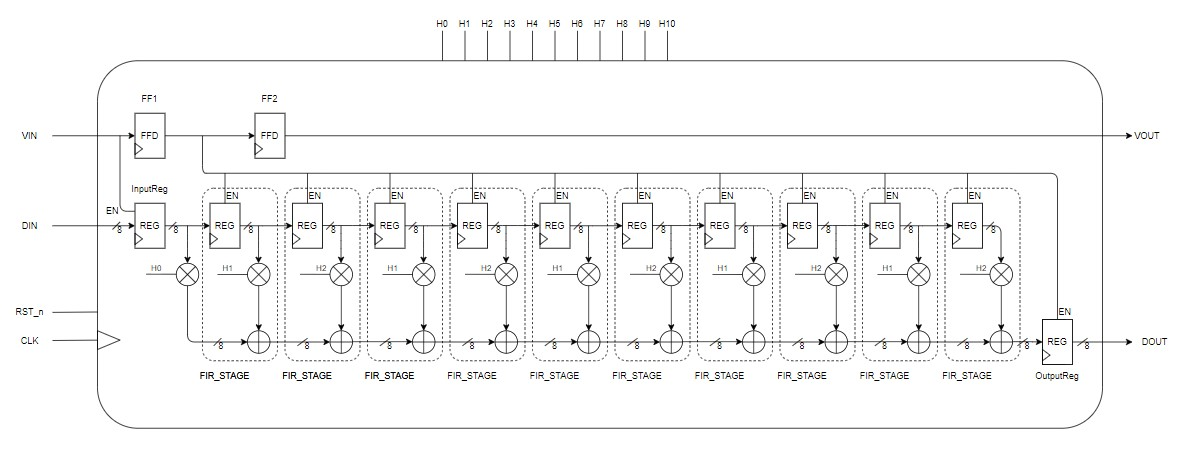
\includegraphics[width=15.5cm]{./chapters/figures/fir_base.jpg}} 

\section{Simulation}

The design was simulated using a testbench written in both Verilog and VHDL. The testbench is composed of four disinct entities:

\begin{itemize}
    \item \textbf{clk\_gen:} generates a clock signal of the specified frequency, and a reset signal.
    \item \textbf{data\_maker:} reads the samples.txt file and provides an input every clock cycle and its validity using the VIN signal. 
    \item \textbf{data\_sink:} recives the outputs of the filter every clock cycle and writes them in the output.txt file if VOUT is equal to 1. 
    \item \textbf{tb\_fir:} is the testbench top entity written in Verilog.
\end{itemize}

\centerline{
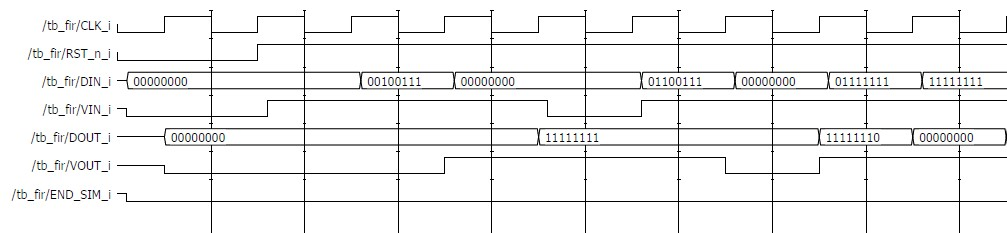
\includegraphics[width=15.5cm]{./chapters/figures/waveform1.jpg}}

\vspace{5mm}
The image above shows an extract of the Modelsim simulation; the waveforms show the moment where VIN goes to zero, and after two clock cycles VOUT is set to zero
in order to avoid errors in the output signal.
At the end of the simulation the values stored in Output.txt were compared with the ones produced by the C prototype. The two files are equal, which
means that the filter is behaving correctly. 

%%table with first results of files
\section{Logic synthesis}
After the simulation the design must be synthetized. To estimate the maximum working clock frequency of the filter,
the clock period in the design compiler is set to 0 ns. In this way the compiler optimizes the circuit as much as possible,
and the negative slack of the timing report corresponds to the maximum clock frequency. 

After running the synthesis at the computed frequency the area is evaluated.\\

%%table with frequency & area
\centerline{
\begin{tabularx}{1\textwidth} { 
    | >{\centering\arraybackslash}X 
    | >{\centering\arraybackslash}X 
    | >{\centering\arraybackslash}X | }
   \hline
   \textbf{Max Clock Frequency} & \textbf{Min Clock Period} & \textbf{Area} \\
   \hline
   303 MHz  & 3.3 ns  & \unit{3765.23}{\micro\meter\squared}  \\
  \hline
\end{tabularx}}
\vspace{5mm}
It is requested to set the frequency to 25\% of the maximum value.

\[ \frac{1}{4} f_{MAX} = 75.75 MHz\]
After the synthesis a new area estimation is produced.

%%new area

\[ Area = \unit{3682}{\micro\meter\squared}\]
The constraints on the clock have a significant role in the estimation of the area: by allowing the frequency to be lower, 
the size of the circuit will be smaller.

The Design Compiler produces the Verilog netlist of the synthetized circuit and a .sdf file containing the circuit's delays.
Those files are used by Modelsim to simulate the netlist with the correct timing parameters and obtain the switching activity of the nodes,
which is saved in a .vcd file. The results of this simulation have been checked to assure that they are coherent with the ones of the
original circuit.

This file is converted to .saif and used by Design Compiler to generete a power report.
\vspace{5mm}
%table with power

\centerline{
\begin{tabularx}{1\textwidth} { 
    | >{\centering\arraybackslash}X 
    | >{\centering\arraybackslash}X 
    | >{\centering\arraybackslash}X
    | >{\centering\arraybackslash}X | }
   \hline
   \multicolumn{4}{|c|}{\textbf{Power [\unit{\micro\watt}]}} \\
   \hline
   \textbf{Internal} & \textbf{Switching} & \textbf{Internal} & \textbf{Total}\\
   \hline
   300.8059  & 252.0369  & 76.517 & 629.3596 \\
  \hline
\end{tabularx}}


\section{Place \& Route}

The last section requires to perform the place and route on the synthetized circuit to obtain the switching activity and power report.
To do that using Innovus several steps are necessary: 

\begin{itemize}
    \item \textbf{Structuring the floorplan}, where Innovus allocates the area for the cells;
    \item \textbf{Inserting power rings}, two rings for power (VDD) and ground (VSS) are inserted around the floorplan;  
    \item \textbf{Standard cell power routing}, horizzontal wires for power and ground are prepared for the cells;
    \item \textbf{Placement}, the cells are placed in the floorplan but are still to be connected between them;
    \item \textbf{Post Clock-Tree-Synthesis optimization}, the design is optimized to achieve the required timing constraints;
    \item \textbf{Place filler}, filler cells are placed to ensure continuity in n+ and p+ wells in each row;
    \item \textbf{Routing}, the cells are connected among each other;
    \item \textbf{Post routing optimization}, the design is optimized again to achieve the timing constraints. After this step, the design is saved as a .enc file;
    \item \textbf{Parasitics extraction}, Innovus extracts the parasitic values of resistencies and capacitances;
    \item \textbf{Timing analysis}, the performance of the circuit is evaluated, if the slack is negative the constraints are violated;
    \item \textbf{Design analysis and verification}, Innovus checks for the presence of floating wires and violations on the constraints on the geometric features of the circuit. 
    Finally the area and gate count, the netlist and a file with delay annotations are saved.
\end{itemize}

%%immagine place&route

\centerline{
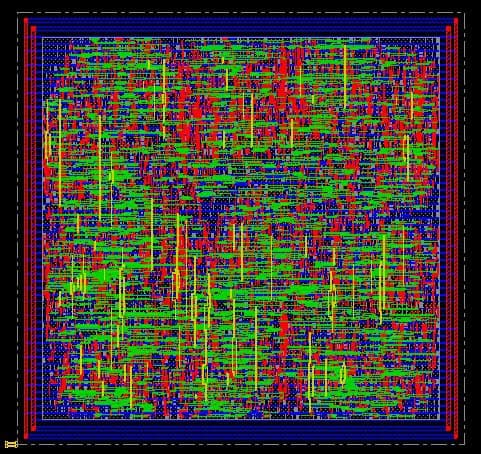
\includegraphics[width=8cm]{./chapters/figures/fir_base_plcrt.jpg}}

\vspace{5mm}

Since the slack values for setup and hold are positive and the verification on connectivity and geometry returned no errors, the final step is to simulate the
produced netlist with Modelsim, to check if the circuit behaves correctly and to calculate the switching activity. The following results have been obtained:
\vspace{5mm}
%tabella con power

\centerline{
\begin{tabularx}{1\textwidth} { 
    | >{\centering\arraybackslash}X 
    | >{\centering\arraybackslash}X 
    | >{\centering\arraybackslash}X 
    | >{\centering\arraybackslash}X | }
    \hline
    \multicolumn{4}{|c|}{\textbf{Power [\unit{\micro\watt}]}} \\
    \hline
    \textbf{Internal} & \textbf{Switching} & \textbf{Internal} & \textbf{Total}\\
    \hline
    207.5  & 175.1  & 73.98 & 516.5 \\
   \hline
\end{tabularx}}
\vspace{5mm}

%tabella con area

\centerline{
\begin{tabularx}{0.6\textwidth} { 
    | >{\centering\arraybackslash}X 
    | >{\centering\arraybackslash}X 
    | >{\centering\arraybackslash}X | }
   \hline
   \textbf{Gates} & \textbf{Cells} & \textbf{Area} \\
   \hline
   4488  & 1874  & \unit{3582}{\micro\meter\squared}  \\
  \hline
\end{tabularx}}
\vspace{5mm}

After the place and route phase, both the area and the power consumption estimations are reduced wth respect to the
ones obtained after the synthesis. This is possible due to the numerous steps of optimization that Innovus performs
on the circuit's netlist.